\section{\Large PROBLEM SET 3}
\subsection{Problem 3}

\subsubsection{Impose that satellite is axial-symmetric (i.e., impose $I_x=I_y\neq I_z$). Repeat numerical simulation from previous pset using initial condition 4) from previous pset.}

The principal inertia of the Aqua satellite is listed in \ref{sec:principal_inertia_def_and_calc}. Imposing that $I_y=I_x$, the axis-symmetric representation of the satellite is seen below.

\begin{equation*}
    \boldsymbol{I_{CM}'} = \begin{bmatrix}
        17510 & 0 & 0 \\
        0 & 17510 & 0 \\
        0 & 0 & 36245
    \end{bmatrix} \text{kg} \cdot \text{m}^2
\end{equation*}

The torque-free simulation results can be seen in Figure \ref{fig:axis_symmetric_magnitudes}.

\subsubsection{Program analytical solution for axial-symmetric satellite. Compute it at same time steps and from same initial conditions.}

The analytical solution for an axis symmetric satellite in torque-free motion comes from Equations \ref{eq:axis_symmetric_1} -- \ref{eq:axis_symmetric_3}.
\begin{eqnarray}
    I_x \dot{\omega}_x + (I_z - I_x) \omega_y \omega_z &= 0 \label{eq:axis_symmetric_1}\\
    I_y \dot{\omega}_y + (I_x - I_z) \omega_z \omega_x &= 0 \label{eq:axis_symmetric_2}\\
    I_z \dot{\omega}_z &= 0 \label{eq:axis_symmetric_3}
\end{eqnarray}
An immediately apparent conclusion is that $\omega_z$ remains constant. That is, $\omega_z = \omega_{z,0}$. Let $\lambda = (I_z - I_x) \omega_{z,0}/ I_x$. This results in the following relations.
\begin{eqnarray*}
    \dot{\omega}_x + \lambda \omega_y &= 0 \\
    \dot{\omega}_y - \lambda \omega_x &= 0
\end{eqnarray*}
Two conclusion can be pulled from this. The first is that $\omega_x^2 + \omega_y^2 = \text{const}$. That is, the norm of the 2D vector composed of x and y components of the angular velocity of the spacecraft is constant. Furthermore, the claim can be made that this vector rotations about the z-axis at a rate of $\lambda$ given in radians per second. The evolution of the x and y components of angular velocity over time given initial conditions $\omega_x (t = 0) = \omega_{x,0}$ and $\omega_y (t = 0) = \omega_{y,0}$ are shown below.
\begin{eqnarray*}
    \omega_x(t) &= \omega_{x,0} \cos{\lambda t} - \omega_{y,0} \sin{\lambda t} \\
    \omega_y(t) &= \omega_{x,0} \sin{\lambda t} + \omega_{y,0} \cos{\lambda t}
\end{eqnarray*}
Therefore the overall vector valued solution is seen in Equation \ref{eq:axis_symmetric_result}.

\begin{equation} \label{eq:axis_symmetric_result}
    \vec{\omega}(t) = \begin{bmatrix}
        \omega_{x,0} \cos{\lambda t} - \omega_{y,0} \sin{\lambda t} &
        \omega_{x,0} \sin{\lambda t} + \omega_{y,0} \cos{\lambda t} & \omega_{z,0}
    \end{bmatrix}^T
\end{equation}

The results of this equation evaluated at the same time steps as the simulation can also be seen in \ref{fig:axis_symmetric_magnitudes}

The

\subsubsection{Compare numerical and analytical solutions. Plot differences (errors), do not only superimpose absolute values. Tune numerical integrator for large discrepancies. Are angular velocity vector and angular momentum vector changing according to theory in principal axes?}

The vector components for both the simulated results and analytical results for axis-symmetric torque-free motion of the Aqua satellite are presented in Figure \ref{fig:axis_symmetric_magnitudes}

\begin{figure} [H]
    \centering
    \captionsetup{justification = centering}
    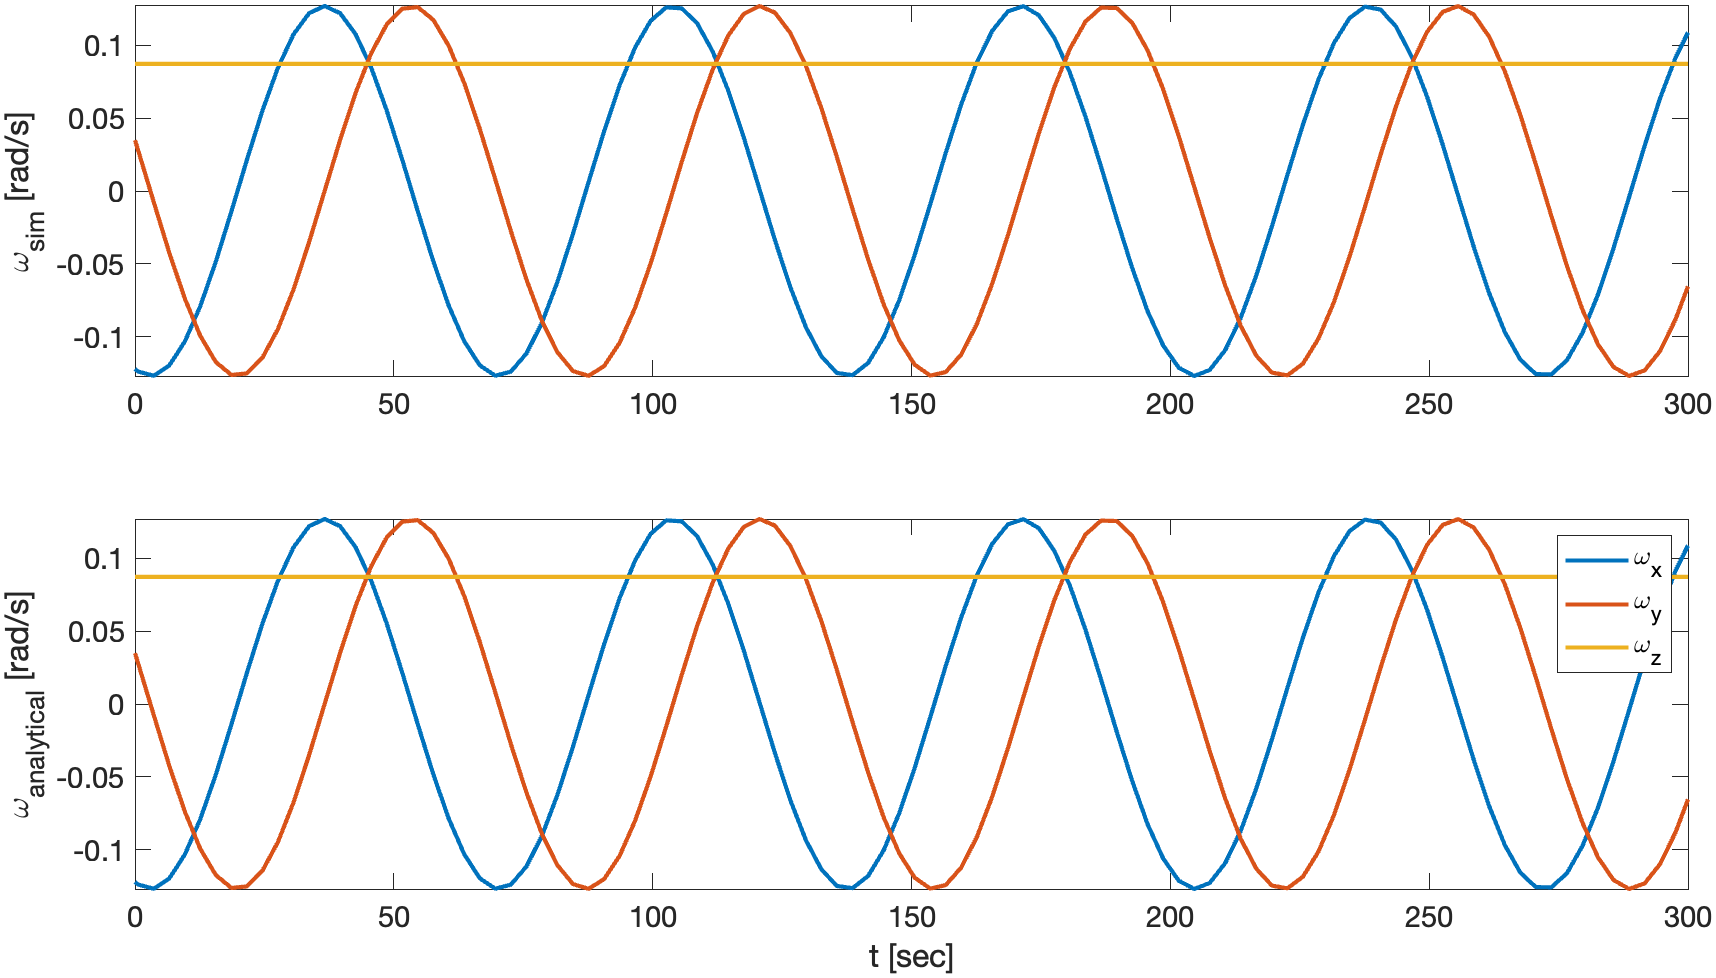
\includegraphics[width = 10cm] {Images/sim_vs_anlt_magnitude.png}
    \caption{Angular Velocity Vector Components for Axis-Symmetric Torque-Free Motion over Time for Simulation (top) and Analytical (bottom) Solutions}
    \label{fig:axis_symmetric_magnitudes}
\end{figure}

\subsubsection{Program Kinematic equations of motion correspondent to a nominal attitude parameterization of your choice.}

\subsubsection{Program Kinematic equations of motion correspondent to a different attitude parameterization from the previous step. This is used for comparison, to get familiar with different approaches, and as fall back solution in the case of singularities.}

\subsubsection{Go back to your original satellite inertia tensor. Numerically integrate Euler AND Kinematic equations from arbitrary initial conditions (warning: stay far from singularity of adopted parameterization). Multiple revolutions. The output is the evolution of the attitude parameters over time. These attitude parameters describe orientation of principal axes relative to inertial axes.}

\subsubsection{Since inertial position, velocity, and attitude, are known at the same time throughout the simulation, it is now possible to express vectors in the reference systems of interest}